
% ----------------------------------------------------------------------
%  Set the document class
% ----------------------------------------------------------------------
\documentclass[11pt,a4paper,twoside]{article}

% ----------------------------------------------------------------------
% Define external packages, language, margins, fonts and new commands
% ----------------------------------------------------------------------
%\input{preamble} 
\usepackage[utf8]{inputenc}   % <<<<< Linux
\usepackage[english]{babel} % <<<<< English
\usepackage{notoccite}
\usepackage[skip=0.5\baselineskip]{caption}
\hyphenation{GTKWave}
\usepackage{listings}
\usepackage[all]{nowidow}

%blind text
\usepackage{lipsum}

\usepackage{comment} % comment out large bodies of text

\usepackage{graphicx}
\graphicspath{ {./} {../../figlib/} }
\def\FontLn{% 16 pt normal
  \usefont{T1}{phv}{m}{n}\fontsize{16pt}{16pt}\selectfont}
\def\FontLb{% 16 pt bold
  \usefont{T1}{phv}{b}{n}\fontsize{16pt}{16pt}\selectfont}
\def\FontMn{% 14 pt normal
  \usefont{T1}{phv}{m}{n}\fontsize{14pt}{14pt}\selectfont}
\def\FontMb{% 14 pt bold
  \usefont{T1}{phv}{b}{n}\fontsize{14pt}{14pt}\selectfont}
\def\FontSn{% 12 pt normal
  \usefont{T1}{phv}{m}{n}\fontsize{12pt}{12pt}\selectfont}

% Use Arial font as default
%
\renewcommand{\rmdefault}{phv}
\renewcommand{\sfdefault}{phv}
\usepackage{geometry}	
\geometry{verbose,tmargin=2.5cm,bmargin=2.5cm,lmargin=2.5cm,rmargin=2.5cm}

%\usepackage{setspace}
%\renewcommand{\baselinestretch}{1.5}

\usepackage[pdftex]{hyperref} % enhance documents that are to be
                              % output as HTML and PDF
\hypersetup{colorlinks,       % color text of links and anchors,
                              % eliminates borders around links
%            linkcolor=red,    % color for normal internal links
            linkcolor=black,  % color for normal internal links
            anchorcolor=black,% color for anchor text
%            citecolor=green,  % color for bibliographical citations
            citecolor=black,  % color for bibliographical citations
%            filecolor=magenta,% color for URLs which open local files
            filecolor=black,  % color for URLs which open local files
%            menucolor=red,    % color for Acrobat menu items
            menucolor=black,  % color for Acrobat menu items
%            pagecolor=red,    % color for links to other pages
            pagecolor=black,  % color for links to other pages
%            urlcolor=cyan,    % color for linked URLs
            urlcolor=black,   % color for linked URLs
	          bookmarks=true,         % create PDF bookmarks
	          bookmarksopen=false,    % don't expand bookmarks
	          bookmarksnumbered=true, % number bookmarks
	          pdftitle={report},
            pdfauthor={Conanga, H.P.},
%            pdfsubject={Thesis Title},
%            pdfkeywords={Thesis Keywords},
            pdfstartview=FitV,
            pdfdisplaydoctitle=true}

\usepackage[numbers,sort&compress]{natbib} % <<<<< References in numbered list [1],[2],...
\usepackage{subcaption} 
\usepackage{mdframed}
\usepackage{amsmath} % facilitates writing math formulas and improves the typographical quality of their output
\usepackage{siunitx} % facilitates writing SI units, along with other SI unit related features
\setcounter{MaxMatrixCols}{20} % enables latex to make matrices w/ 20 columns


%%%%%%%%%%%%%%%%%%%%%%%%%%%%%%%%%%%%%%%%%%%%%%%%%%%%%%%%%%%%%%%%%%%%%%%%
%     Begin Document                                                   %
%%%%%%%%%%%%%%%%%%%%%%%%%%%%%%%%%%%%%%%%%%%%%%%%%%%%%%%%%%%%%%%%%%%%%%%%


\begin{document}

% Set plain page style (no headers, footer with centered page number)
\pagestyle{plain}

% Set roman numbering (i,ii,...) before the start of chapters
%\pagenumbering{roman}

% ----------------------------------------------------------------------
%  Cover page
% ----------------------------------------------------------------------
%%%%%%%%%%%%%%%%%%%%%%%%%%%%%%%%%%%%%%%%%%%%%%%%%%%%%%%%%%%%%%%%%%%%%%%%
%                                                                      %
%     File: Thesis_FrontCover.tex                                      %
%     Tex Master: Thesis.tex                                           %
%                                                                      %
%     Author: Andre C. Marta                                           %
%     Last modified :  2 Jul 2015                                      %
%                                                                      %
%%%%%%%%%%%%%%%%%%%%%%%%%%%%%%%%%%%%%%%%%%%%%%%%%%%%%%%%%%%%%%%%%%%%%%%%

\thispagestyle {empty}

% IST Logo - Signature A
% parameters: bb=llx lly urx ury (bounding box), width=h_length, height=v_length, angle=angle, scale=factor, clip=true/false, draft=true/false. 
%\includegraphics[bb=9.5cm 11cm 0cm 0cm,scale=0.29]{IST_A_CMYK_POS}

\begin{center}
%
% Figure (Image or plot)
\vspace{1.0cm}
% height = 50 mm
%\includegraphics[height=50mm]{Figures/Airbus_A350.jpg}

% Title, author and degree
\vspace{1cm}
{\FontLb Circuit Theory and Electronics Fundamentals} \\ % <<<<< EDIT TITLE
\vspace{1cm}
{\FontSn BSc Aerospace Engineering, Técnico, University of Lisbon} \\ % <<<<< EDIT COURSE
\vspace{1cm}
{\FontSn Lab 4: Audio Amplifier} \\
\vspace{1cm}
{\FontSn May 23, 2021} \\ % <<<<< EDIT DATE (corresponds to date of oral examination)
\vspace{1cm}
{\FontSn Group 48} \\ %group
{\FontSn Dinis Papinha, 84379} \\ %authors
{\FontSn Filipa Gonçalves, 89662} \\ %authors
{\FontSn Carlos de Vasconcelos, 90227} \\ %authors
%
\end{center}


% ----------------------------------------------------------------------
% Dedication page (optional)
% ----------------------------------------------------------------------
%\input{dedication} 
%\cleardoublepage

% ----------------------------------------------------------------------
%  Acknowledgments (optional)
% ----------------------------------------------------------------------
%\input{acknowledgements}
%\cleardoublepage

% ----------------------------------------------------------------------
%  Abstract (both in English and Portuguese)
% ----------------------------------------------------------------------
%\input{resumo} 
%\cleardoublepage

%\input{abstract} 

% ----------------------------------------------------------------------
%  Table of contents, list of tables, list of figures and nomenclature
% ----------------------------------------------------------------------

% Table of contents
%
\tableofcontents

% List of tables
%\addcontentsline{toc}{section}{\listtablename}
%\listoftables
%\cleardoublepage 

% List of figures
%\addcontentsline{toc}{section}{\listfigurename}
%\listoffigures
%\cleardoublepage 

% Set arabic numbering (1,2,...) after preface
%
%\setcounter{page}{1}
%\pagenumbering{arabic}

% ----------------------------------------------------------------------
%  Body
% ----------------------------------------------------------------------

\section{Introduction}
\label{sec:introduction}

% state the learning objective 
The objective of this laboratory assignment is to analyse and optimize an audio amplifier circuit, with a $12V$ supply voltage (Vcc) and an audio input of up to $10mV$, using a gain and an output stage, as presented in Figure  \ref{fig:circuit}. In order to optimize the circuit, it was possible to manipulate the values of several parameters, which had assigned costs, given by the Professor.. The \textit{Merit} score is obtained as a function of the chosen architecture's cost and the performance of the circuit. 


\begin{figure}[h] \centering
\includegraphics[width=0.9\linewidth]{circuit.pdf}
\caption{Audio amplifier circuit.}
\label{fig:circuit}
\end{figure}

The parameters changed (in relation to the circuit given by the Professor) are given in Section~\ref{sec:analysis}, along with its cost.


In Section~\ref{sec:analysis}, using \textit{Octave}, a theoretical analysis is presented, in which we describe the theoretical model used to analyze the circuit are presented. In this Section's last subsection (Subsection \ref{subsec:theo_merit}), the cost of the circuit and Merit score are determined. In Section~\ref{sec:simulation}, the circuit is analyzed by simulation, but using the Ngspice software. The results are compared in Subsection~\ref{subsec:compare} (the last of this third Section). The conclusions of this study are outlined in Section~\ref{sec:conclusion}.


\newpage
\section{Theoretical Analysis}
\label{sec:analysis}

Solvig the OP problem we get $VCE=2.1578$

Regarding the gains plots between the first and 2 stage we can see that they do not differ alot, this is beliveble since AV2=-0.0348 db as we can see in the table, so it does not vary much the result.


\begin{figure}[h]
\centering
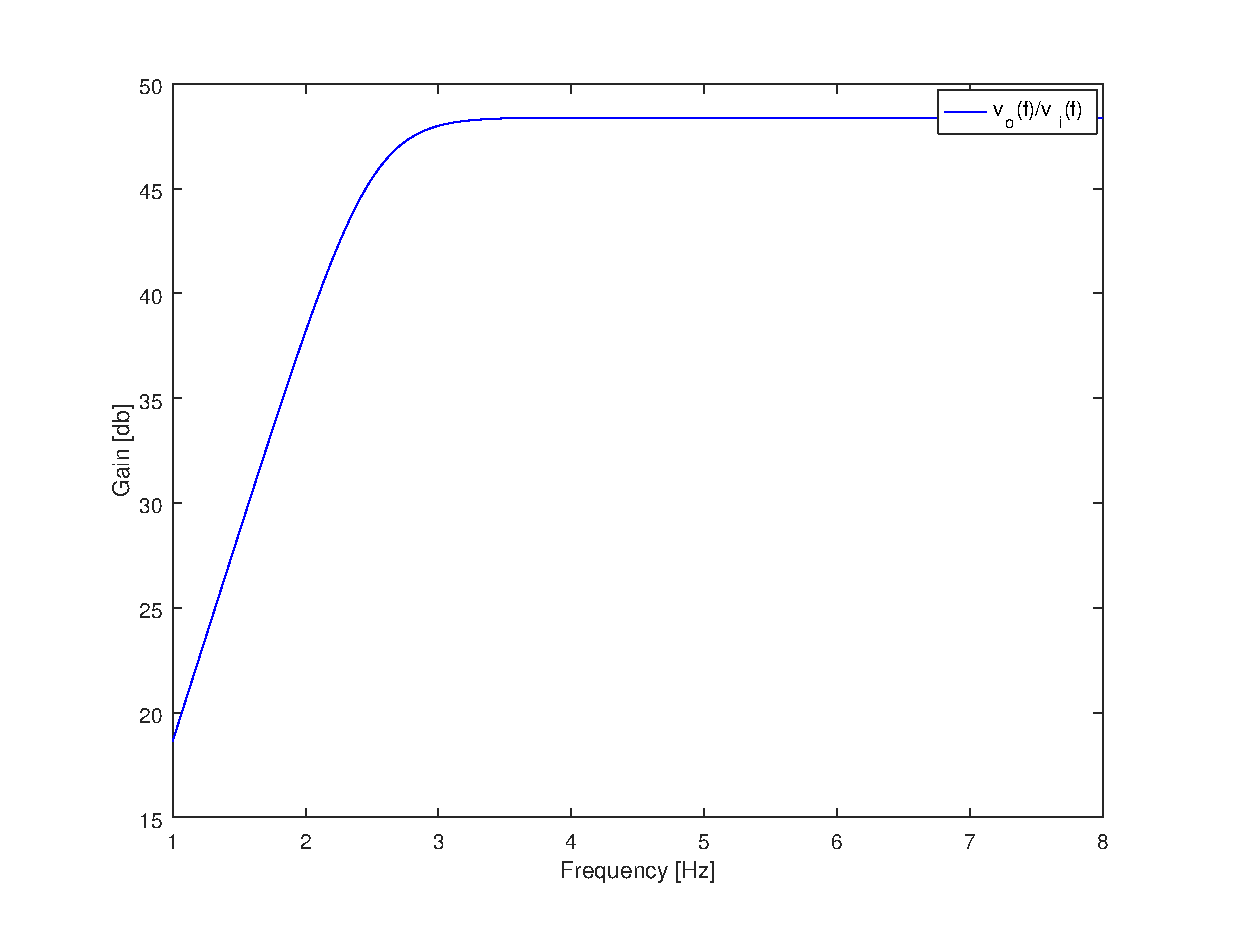
\includegraphics[width=0.6\linewidth]{Gain1.eps}
\caption{Gain in the first phase}
\label{plot:ganho1}
\end{figure}


Nevertheless the inputs and outputs for this stages are present in the following table:


\begin{table}[h]
\begin{tabular}{ll}
AV1 & 262.79 \\
ZI1 & 484.43 \\
Z01 & 886.28 \\
AV2 & 0.996  \\
ZI2 & 8598.9 \\
Z02 & 0.302 
\end{tabular}
\end{table}

\newpage

As such the final gain plot can be given by the following Figure.
\begin{figure}[h]
\centering
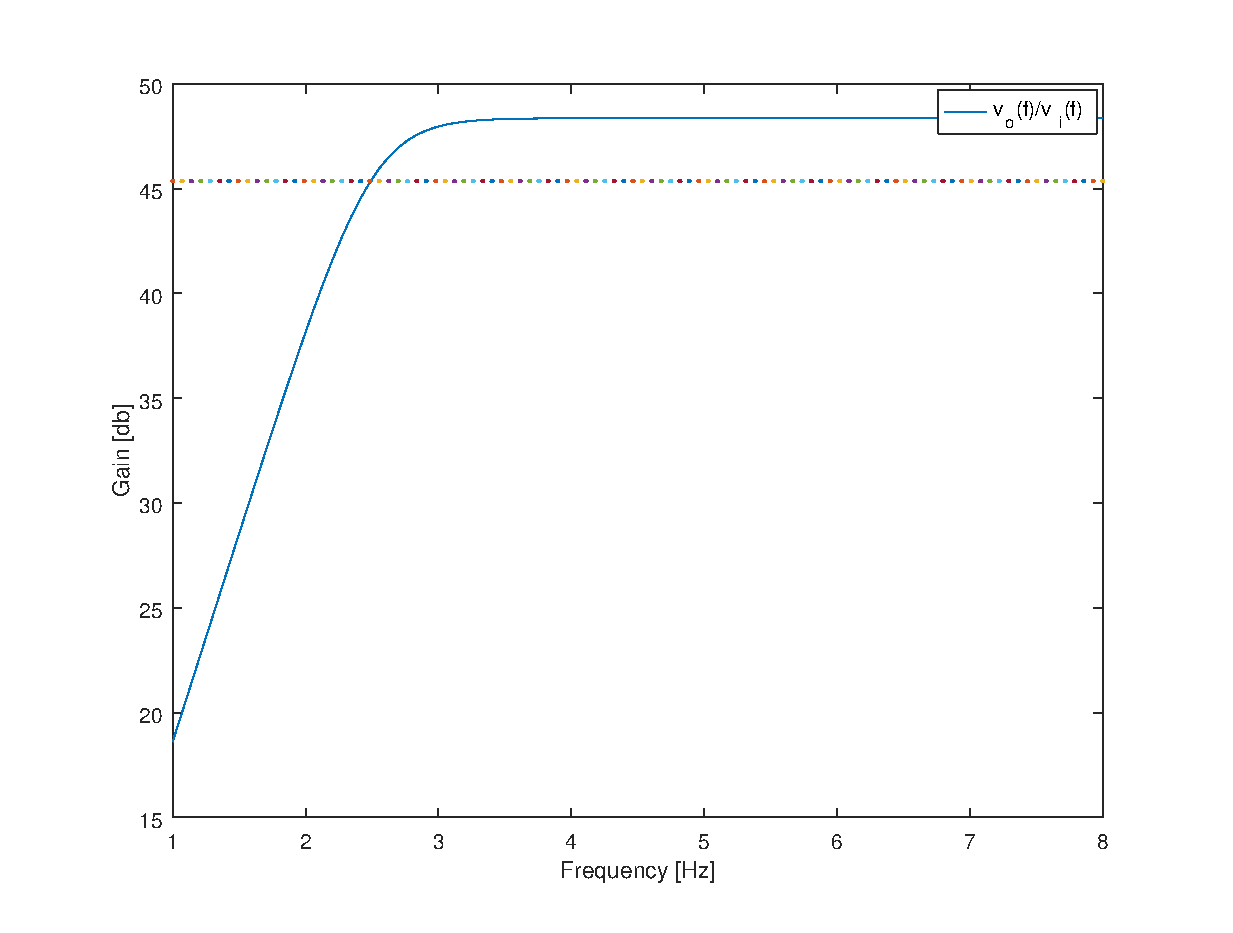
\includegraphics[width=0.6\linewidth]{GainFinal.eps}
\caption{Output Gain}
\label{plot:ganho2}
\end{figure}




\section{Simulation Analysis}
\label{sec:simulation}

In this section, the intent is to simulate the circuit, using \textit{Ngspice}. 

Firstly, the operation point was obtained and the functioning of the NPN and PNP transistors in the F.A.R was assessed, being concluded in the following tables.

\begin{center}
    \begin{tabular}{|l|r|}
      \hline    
      {\bf Variable} & {\bf Value} \\ \hline
      \input{npn_tab.tex}
    \end{tabular}
\end{center}

And

\begin{center}
    \begin{tabular}{|l|r|}
      \hline    
      {\bf Variable} & {\bf Value} \\ \hline
      \input{PNP_tab.tex}
    \end{tabular}
\end{center}

Then, time and frequency analysis were performed in order to evaluate the collector (coll) and the output (out) voltage gain in the passband, the lower ($f_1$) and the upper ($f_2$) cutoff frequencies, the bandwith (difference between the cutoff frequencies) and the input (Zin) and output (Zout) impedances of the overall circuit. The following plots and tables represent such evaluations, along with the calculation of the cost and merit figure of the circuit.

\begin{figure}[h]
    \centering
    \includegraphics[width=0.5\linewidth]{vo1.pdf}
    \caption{Magnitude db plot for voltage in node coll/collector with time}
    \label{vo1}
\end{figure}

\begin{figure}[h]
    \centering
    \includegraphics[width=0.5\linewidth]{vo1f.pdf}
    \caption{Magnitude db plot for voltage in node coll/collector with frequency}
    \label{vo1f}
\end{figure}

\begin{figure}[h]
    \centering
    \includegraphics[width=0.5\linewidth]{vo2f.pdf}
    \caption{Magnitude db plot for voltage in node out/output with frequency}
    \label{vo2f}
\end{figure}

\clearpage

The tables are 

\begin{center}
    \begin{tabular}{|l|r|}
      \hline    
      {\bf Variable} & {\bf Value} \\ \hline
      \input{measurements_tab.tex}
    \end{tabular}
\end{center}

\begin{center}
    \begin{tabular}{|l|r|}
    \hline    
    {\bf Variable} & {\bf Value} \\ \hline
    \input{Zout_tab.tex}
    \end{tabular}
\end{center}

The parameters aimed to optimize are in the following table once more.

\begin{center}
    \begin{tabular}{|l|r|}
      \hline    
      {\bf Variable} & {\bf Value} \\ \hline
      \input{goals_tab.tex}
    \end{tabular}
\end{center}

Understanding the purpose of the coupling capacitors on our circuit and confirming that understanding by "playing around" (changing their parameter values) on ngspice, it can be infered that the bandwith increases as the capacitance increases, since the lower cutoff frequency ($f_1$) decreases and the higher one ($f_2$) isn't affected. This increase will allow the transistors to keep operating at lower frequencies, since their impedance tends to infinity with $\omega$ approaching 0.

Understanding the purpose of the bypass capacitor on our circuit and confirming that understanding by "playing around" (changing its parameter value) on ngspice, it can be infered that, as its capacitance increases, the first stage gain increases. That is because its impedance is $1/(jwC)$ ($w=2 \pi f$), and it is placed in paralel with a resistance ($R_E$), which varies inversely with the first stage gain. As such, with higher frequencies and capacitance, the impedance diminishes and, gradually, the capacitor starts to work as a short-circuit and to bypass the resistor $R_E$.

Understanding the impact of the $R_C$ on our circuit and confirming that understanding by "playing around" (changing its parameter value) on ngspice, it can be infered that, as $R_C$ increases, the gain also increases, which can be greatly observed with a theorical analysis of the circuit asweel: $R_C$ and the gain of the circuit are proportional.



\section{Conclusion}
\label{sec:conclusion}

Comparing these results given by the NGspice with the ones calculated with the octave we can see a clear difference. Therefore, the Merit considered was the one obtained from the Ngspice software, since the analysis made with octave software doesn't seem that of a passband and the results may be less valid. As such, the gain (for the merit calculation) was obtained with the Ngspice program.
%\cleardoublepage

% ----------------------------------------------------------------------
%  Bibliography
% ----------------------------------------------------------------------
%\addcontentsline{toc}{section}{\bibname}
%\bibliographystyle{abbrvunsrtnat} % <<<<< SELECT IF USING REFERENCES BY NUMBER (CITATION ORDER)
%\bibliography{../../../BIBfile.bib}

% ----------------------------------------------------------------------
\end{document}
% ----------------------------------------------------------------------

